\chapter{A módszer leírása}
\label{ch:method}

A szemantikus reprenzentációs módszerek kutatása intenzíven felgyorsult az elmúlt évtizedben. Bár a szélesebb körben beszélt nyelvek esetében – például angol, kínai – számos technika és adathalmaz is elérhető, a kis és közepes nyelveknek egyelőre nélkülözniük kell ezeket. A probléma  feltehetőleg részben a kutatási terület újszerű jellegéből és a nagy tömegek igényeinek hiányából fakad. 

Ismereteim szerint magyar nyelven a tárgyalt kategóriák közül kizárólag szóbeágyazási modellek léteznek – mint a FastTex, Word2Vec és az ELMo – , továbbá a lehetséges tanítási feladatok is korlátozottak, így többnyire csak felügyelet nélküli tanítás elvégzése lehetséges. A diplomamunkám során megoldandó feladat egy mondat/paragrafus szintű nyelvi modell elkészítése, amely alapjául az előzményekben megismert módszerek szolgálnak. Továbbá olyan humán és autoannotált adathalmazok létrehozása és vizsgálata, melyeket a tanítási folyamathoz használok fel. Az így kapott előre tanított nyelvi modell reményeim szerint alkalmas lesz a későbbi NLP feladatokhoz szükséges finomhangolásra, továbbá a létrehozott adathalmazok és a tanításhoz használt algoritmusok más munkák segítségére is lehetnek.

A feladat megoldására szolgáló módszer alapvetően három részből áll: a bemeneti rétegből, a reprezentáció létrehozásához használt neurális hálóból és a modell tanításához definiált feladatokból, az ehhez alkalmazott fejekből. Mivel a szóalapú megoldások általában pontosabb eredményt mutatnak, mint a karakter, vagy szótöredék alapú modellek, így ebben az esetben is szavak kerülnek feldolgozásra.

\begin{figure}[H]
	\centering
	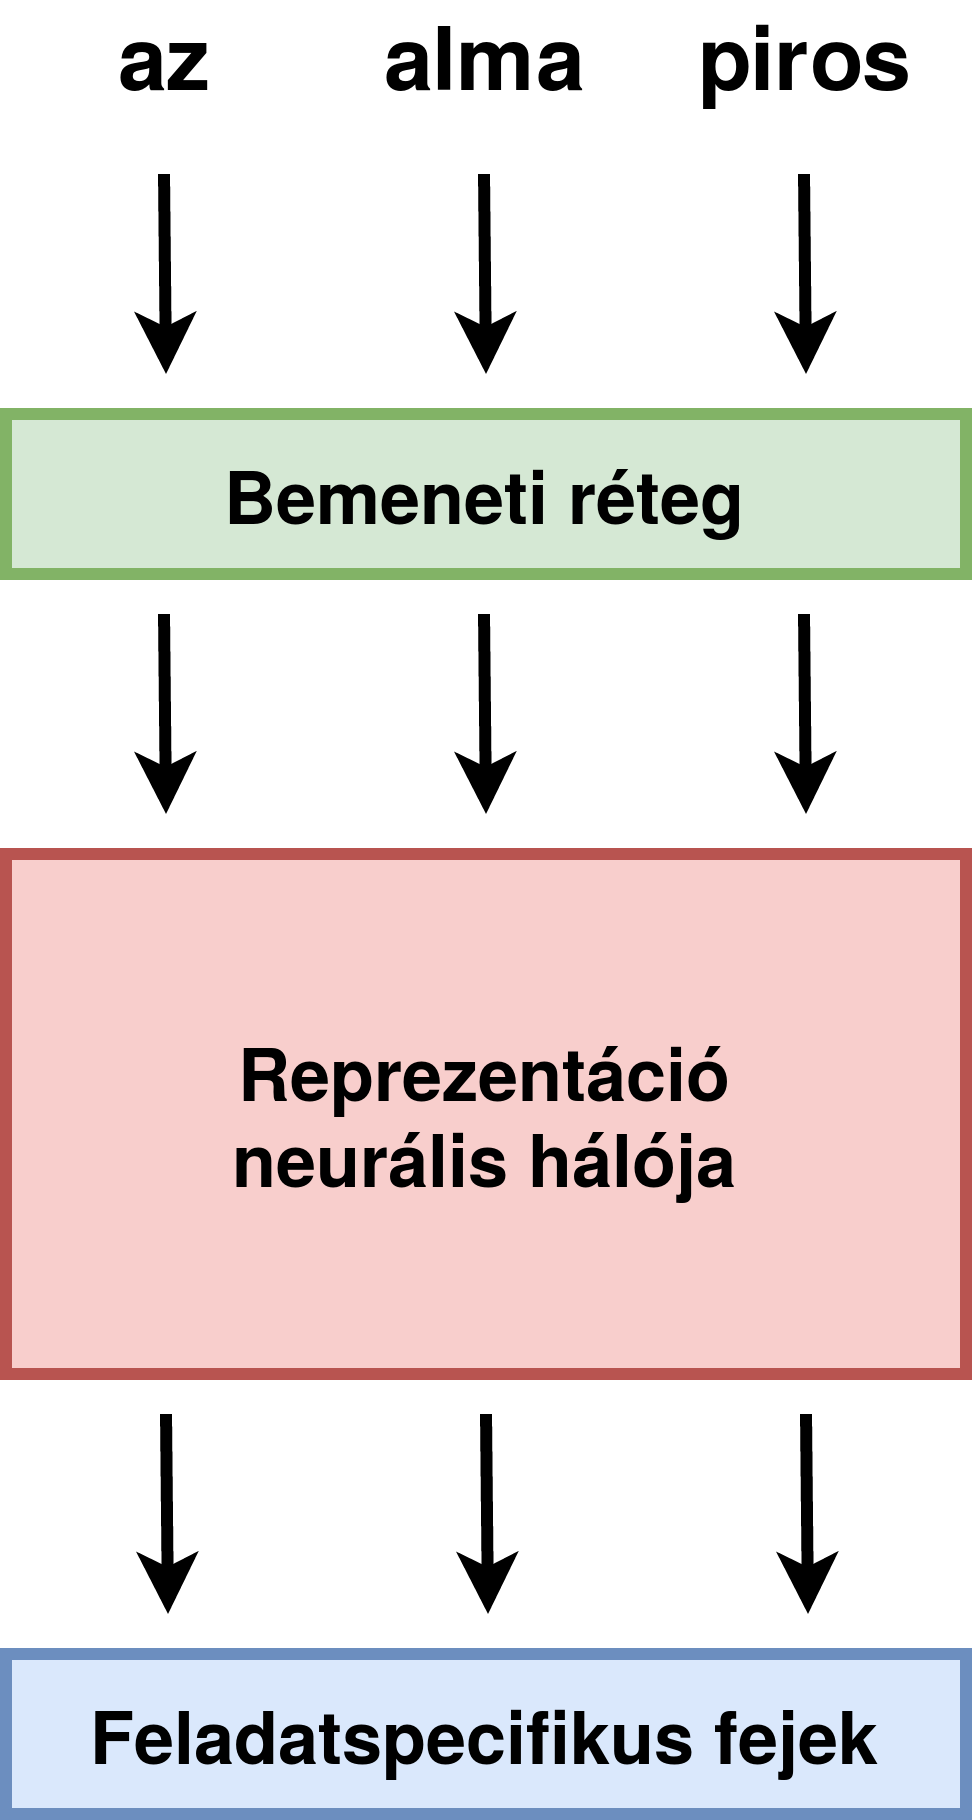
\includegraphics[width=0.3\textwidth,height=220px]{architecture}
	\caption{A módszer magasszintű architektúrája}
\end{figure}

Az implementációt Python nyelven végeztem a Tensorflow nevű könyvtár segítségével.

\section{Bemeneti réteg}

Ahogyan több módszer esetén is láthattuk, előfordulhat, hogy a neurális hálók bemenetére már eleve vektorizált formában érkeznek a token-ek. A feladat megoldásához használt architektúrában az input koordinálását egy bemeneti réteg végzi. Ezen réteg a felhasználó által konfigurálható attól függően, hogy az inputra a token-ek enkódolt formában érkeznek, vagy az algoritmus a számára megadható szóbeágyazási modellt használja. Ha a token-ek nem vektor formájában kerülnek a bemenetre, akkor a bemeneti réteg a token-ekhez rendelt egyedi azonosító számok szekvenciáját fogadja.

A tanítás során minden esetben a mélyháló számára megadott Word2Vec - CBOW szóbeágyazási modelleket használtam, melyek 300 dimenziós szóvektorokat tartalmaznak. A szóbeágyazások tanítóalgoritmusa 5 token széles ablakot alkalmazott. A wiki\_hu 658 129, az oscar modell 2 335 673, az oscar\_sm pedig 645 136 darab vektorból áll. Az előtanítás során átadott reprezentációs mátrixot a GPU a memóriában tárolja és műveleteket is végez vele, ezért a nagyobb, oscar\_hu halmazon tanított modell rendkívül memóriaigényesnek, továbbá a wiki\_hu tanítóhalmaz a Word2Vec tanításához túl kisméretűnek bizonyult, így a végső választás az oscar\_sm modellre esett. 

\begin{figure}[H]
	\centering
	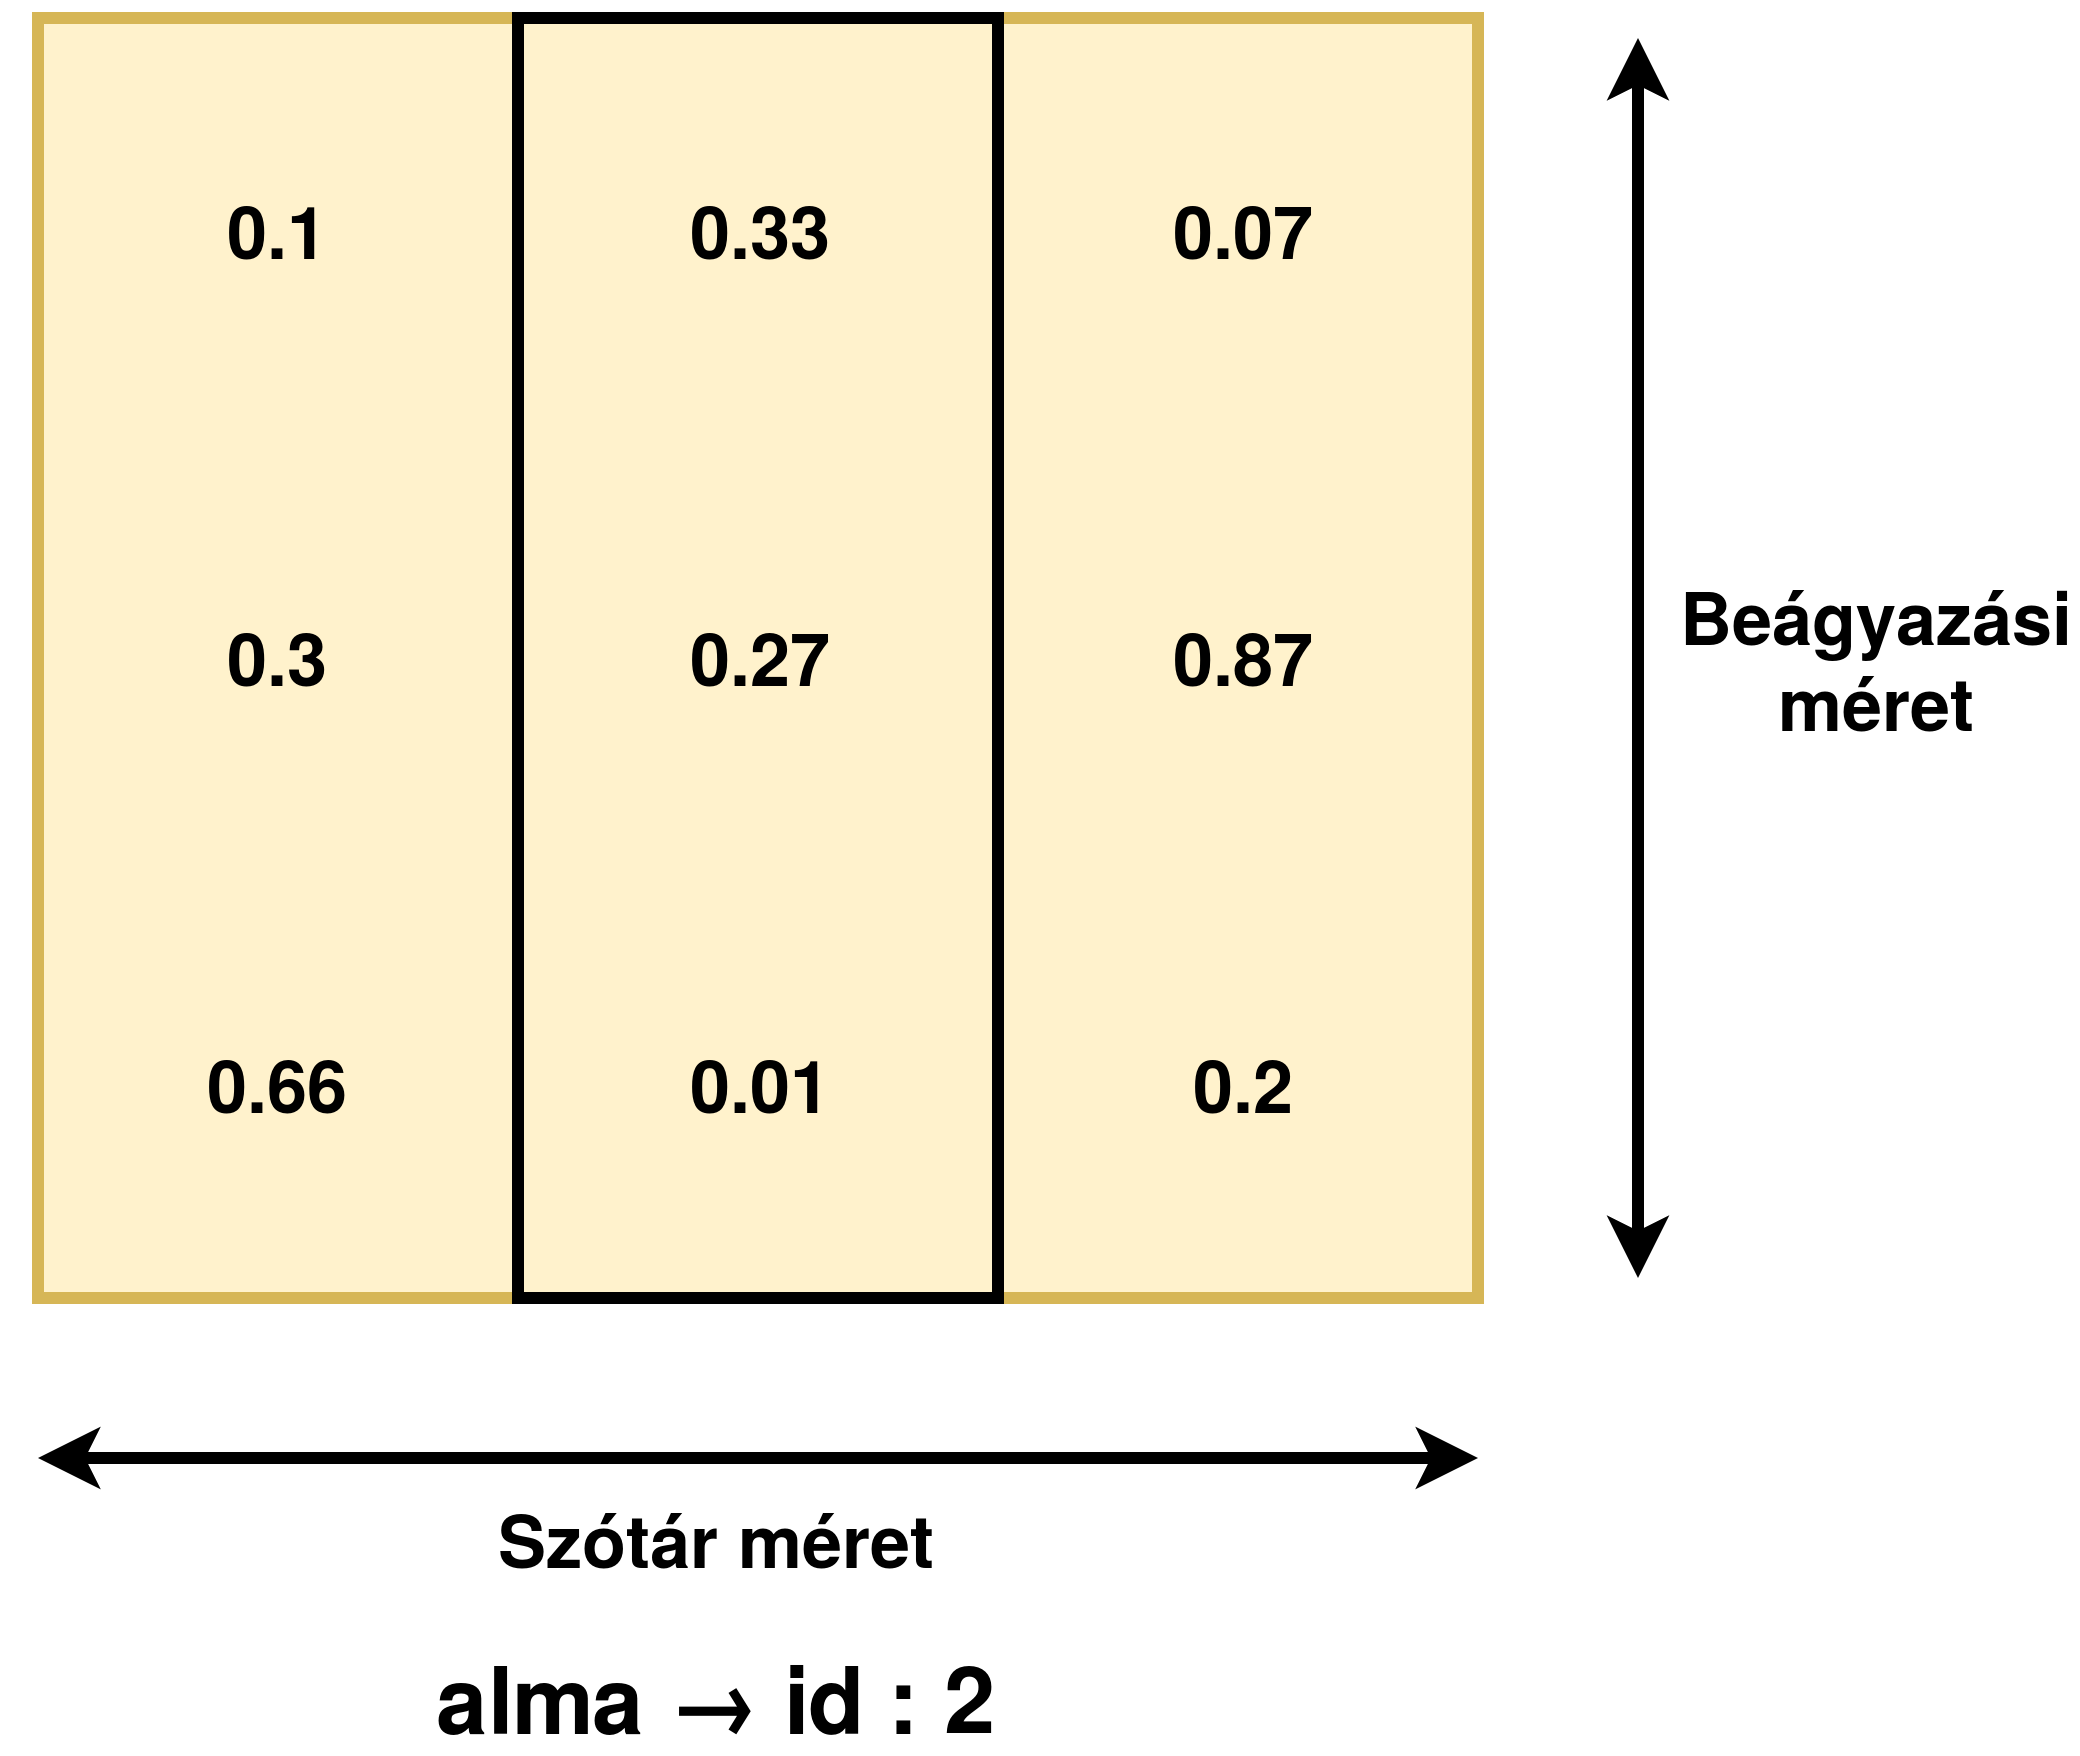
\includegraphics[width=0.6\textwidth,height=220px]{embedding}
	\caption{Az embedding lookup}
\end{figure}

A bemeneti réteg fix súlyokkal rendelkezik, tehát a tanulási folyamat során nem változtatja azokat. A mélyháló a számára átadott beágyazási mátrix elemei közül kikeresi az azonosítóknak megfelelő elemeket, majd továbbítja őket a kimenetre. Ezt a folyamatot \textit{embedding lookup}-nak nevezzük.

\section{A reprezentáció neurális hálója}

A rekurrens neurális hálók (RNN) használata a szemantikus reprezentációs modellek esetén gyakori technika. Míg a mesterséges neurális hálók csak önálló bemenet fogadására képesek, addig a rekurrens neurális hálók alkalmasak szekvenciális input feldolgozására is. Ilyen szekvencia például az idősori adat, vagy a szöveges adat is. A szekvenciális bemenetet az különbözteti meg önálló bemenettől, hogy a szekvenciális input elemei függenek egymástól, hatással lehetnek a szomszéd elemekre, több önálló input esetén ez a reláció nem érvényes.
A rekurrens neurális hálók képesek megtanulni az adatsor elemei közötti kapcsolatokat. Az RNN a tanulási folyamat során "emlékszik" az előző bemenetekből gyűjtött információkra, majd azok segítségével generálja a kimenetet/kimeneteket. A számítás során használt vektorokat nem csak az input súlyai befolyásolják, hanem a rekurrens háló rejtett állapotvektorai is. A rejtett állapot megtanulja a folytonos bemenet elemei közti függőségeket, majd minden tanítási lépés során frissül. Ennélfogva minden egyes bemeneti elem más és más műveleten esik át.

\begin{figure}[H]
	\centering
	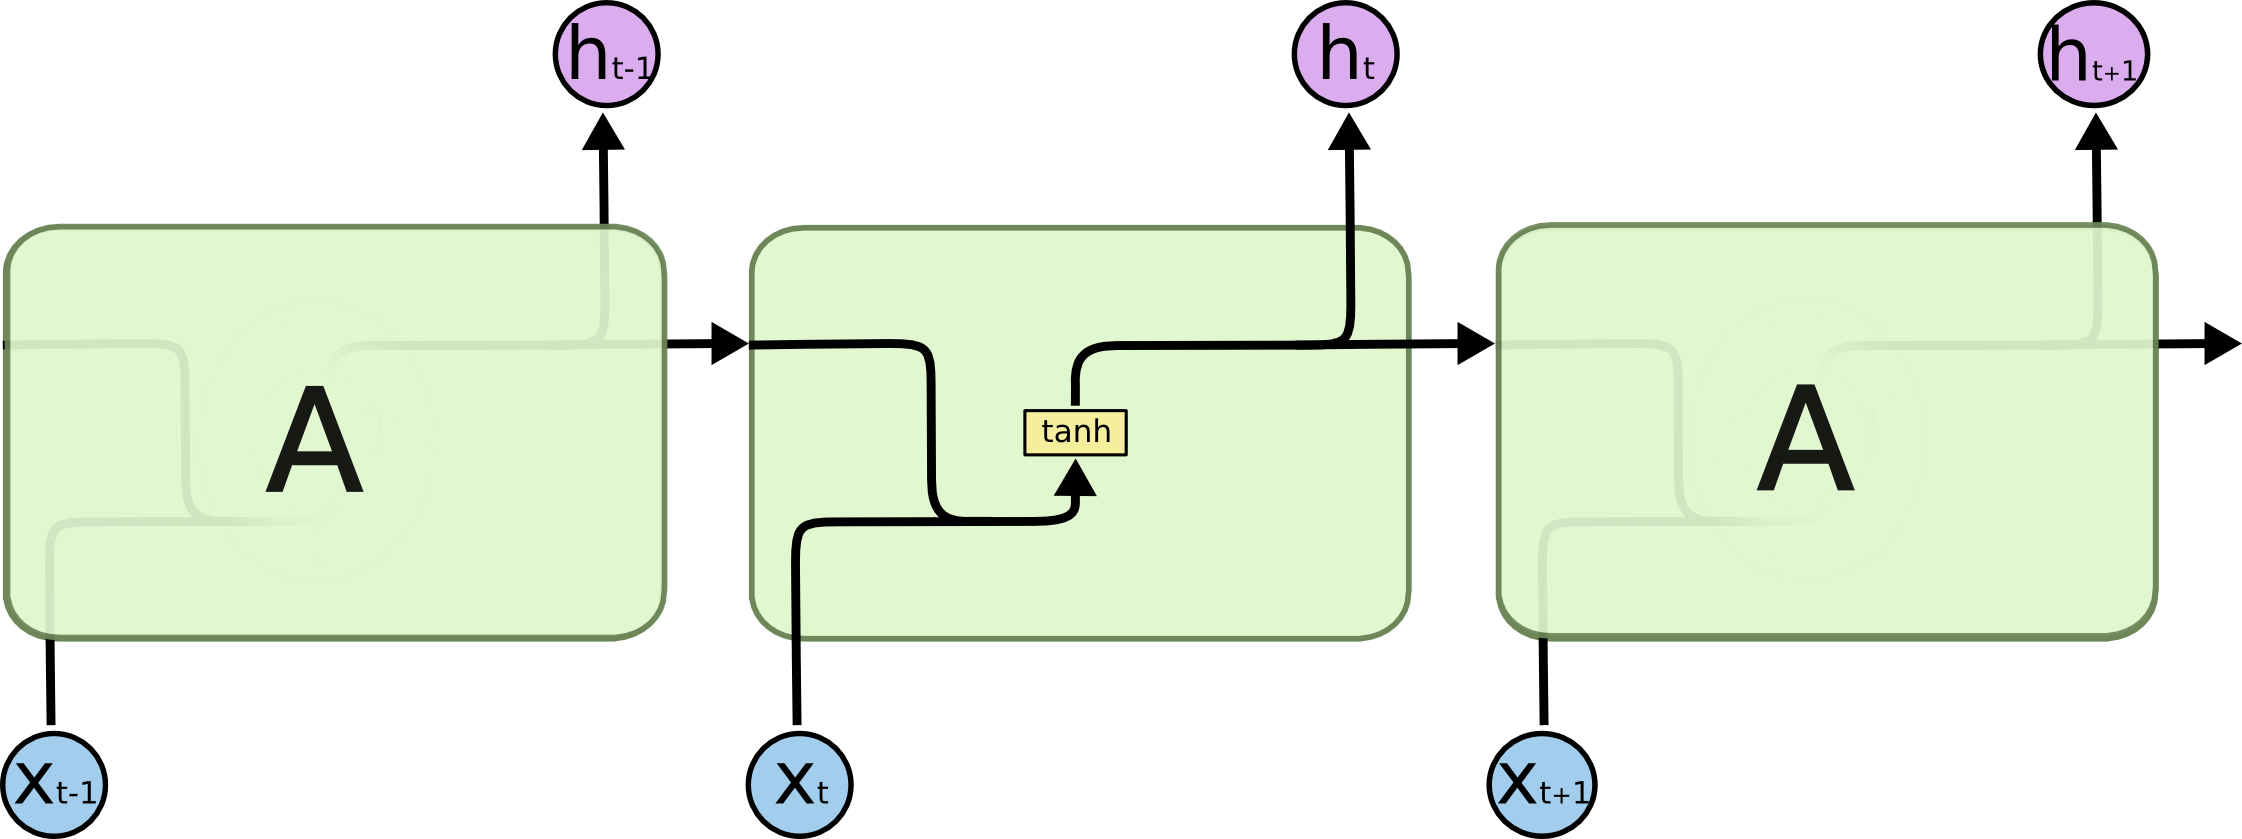
\includegraphics[width=0.55\textwidth,height=100px]{rnn}
	\caption{Az RNN cella}
\end{figure}

Bizonyos esetekben, ahol a múltból származó információ elegendő lehet a háló számára – például következő token generálása az előzőek függvényében – , az RNN jó opció lehet. Azonban olyan feladatok során, melyeknél fontos a bemeneti adatok kontextusa – például a nyelvi modellek – , más megoldásra van szükség. A BiRNN architektúra lényege, hogy az inputot két, egymással ellentétes irányú rekurrens háló olvassa. Az így kapott kimeneti vektorok páronkénti konkatenációja lesz a BiRNN output-ja.

\begin{figure}[H]
	\centering
	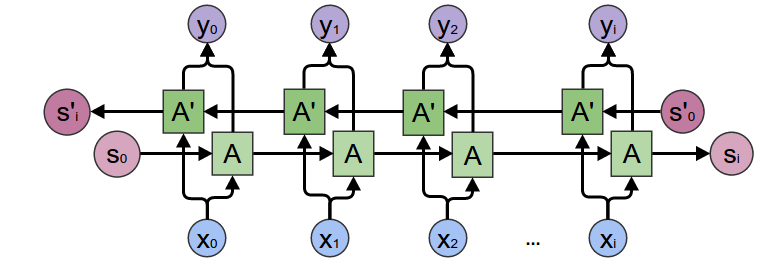
\includegraphics[width=0.7\textwidth,height=120px]{birnn}
	\caption{A BiRNN architektúra}
\end{figure}

Az RNN-ek legegyszerűbb formájának (\textit{Vanilla RNN}) azonban van egy nagy gyengesége, ami a hosszútávú információkat illeti. Gradiensnek hívjuk azokat az értékeket, melyeket a háló a súlyai frissítésére használ. Vanilla RNN esetén a visszaterjesztési művelet (\textit{backpropagation}) alatt annyira lecsökkenhetnek a túl kicsi gradiensek, hogy a hozzá tartozó rétegek megállnak a tanulásban. Ezt a problémát a \textit{vanishing gradients} problémának hívjuk.

Az LSTM (\textit{Long short-term memory}) architektúra megoldást nyújt a \textit{vanishing gradient} problémára. Az LSTM a megszokott hosszútávú memória mellé bevezeti a rövidtávú memóriát is. Olyan belső műveletei vannak, melyek képesek szabályozni az adott cellán belüli információáramlást. Ezen műveleteket kapuknak nevezzük. A kapuk eldönthetik, hogy mely információ lesz fontos a továbbiakban és melyiket lehet törölni. A módszer csak releváns információt enged a hosszútávú memóriába.

\begin{figure}[H]
	\centering
	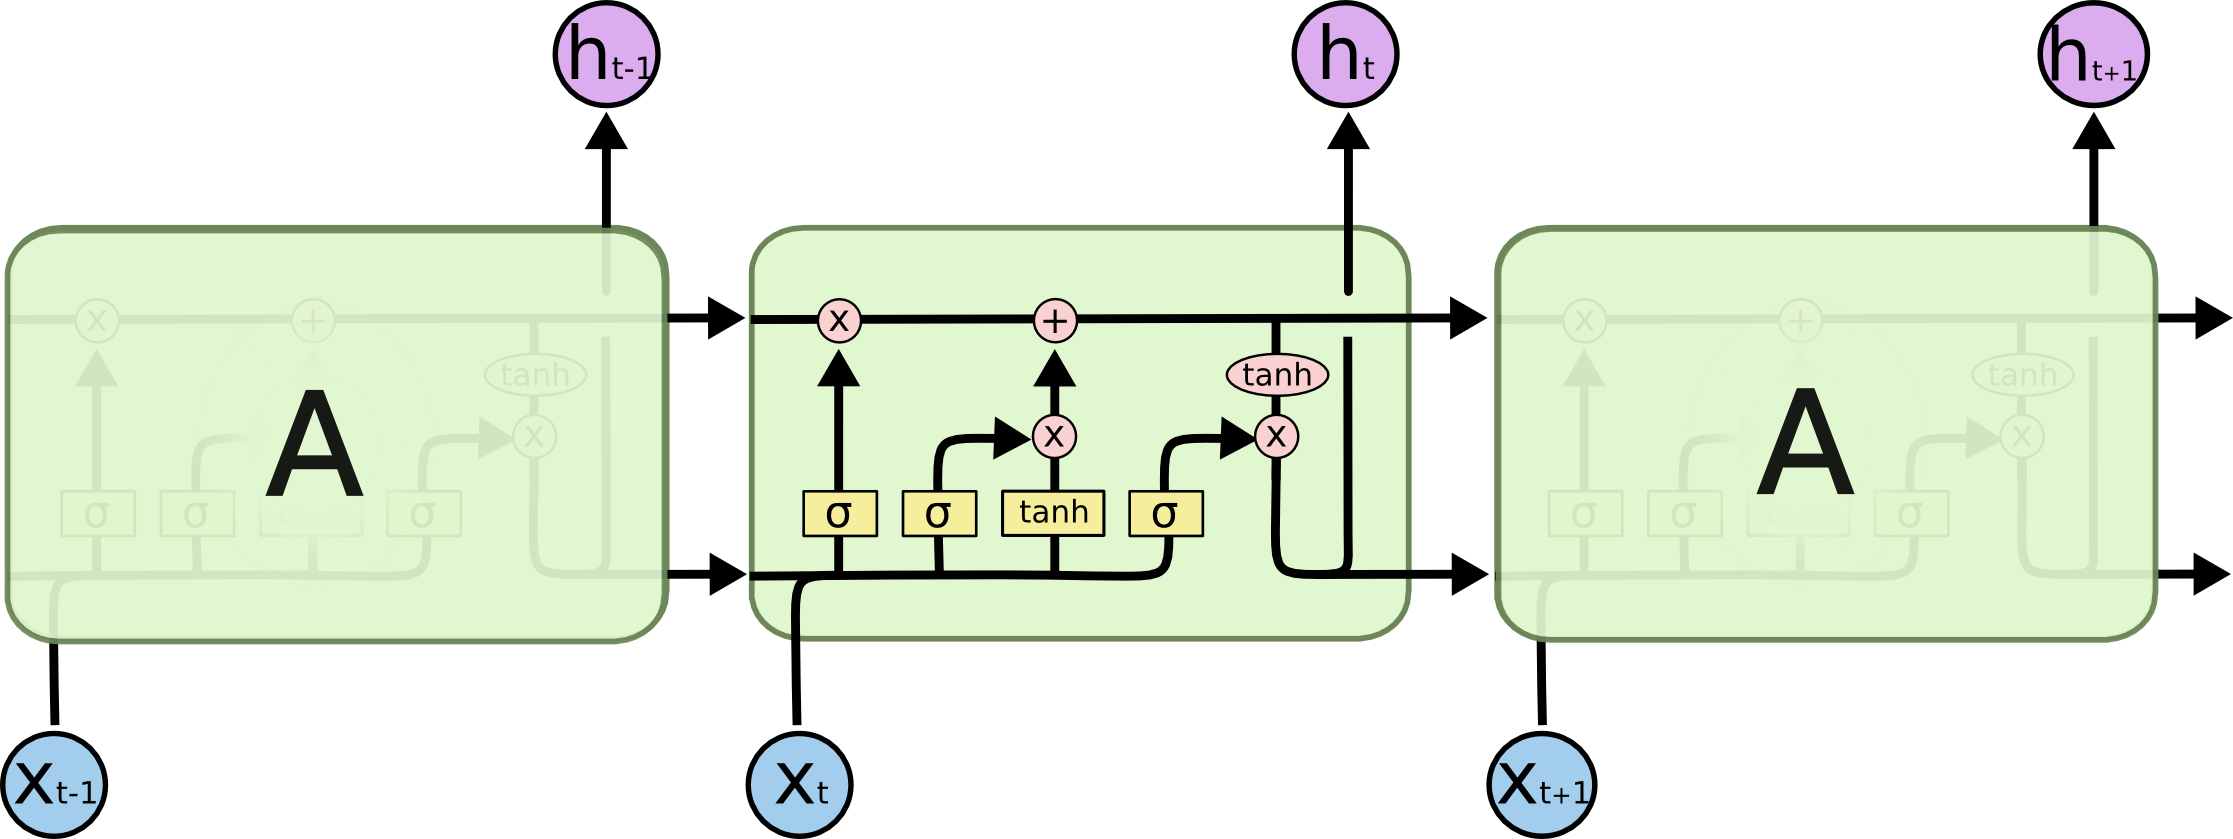
\includegraphics[width=0.55\textwidth,height=100px]{lstm}
	\caption{Az LSTM cella}
\end{figure}

(Írjak még az LSTMről?, kapuk, aktivációk részletesen)

Az általam a feladat megoldására választott architektúra az InferSent-ben kiváló eredményeket prezentáló BiLSTM + Max Pooling.

\subsection{A BiLSTM}
A BiLSTM egy kétirányú rekurrens architektúra (BiRNN), amely LSTM cellákat használ. Az NLP feladatok természetes nyelven írott szöveggel operálnak, így a rekurrens neurális háló az egyik alternatíva a változó hosszúságú szekvenciális adat feldolgozására. A kétirányú modell figyelembe veszi a feldolgozandó token kontextusát a tanulás során és eltárolja a sorrendi információkat is. Az LSTM cellák alkalmazása széles körben elterjedt technika, amely amellett, hogy képes kezelni az RNN gyengeségeit, az egyik jelenlegi legpontosabb megoldásnak bizonyul.

\begin{figure}[H]
	\centering
	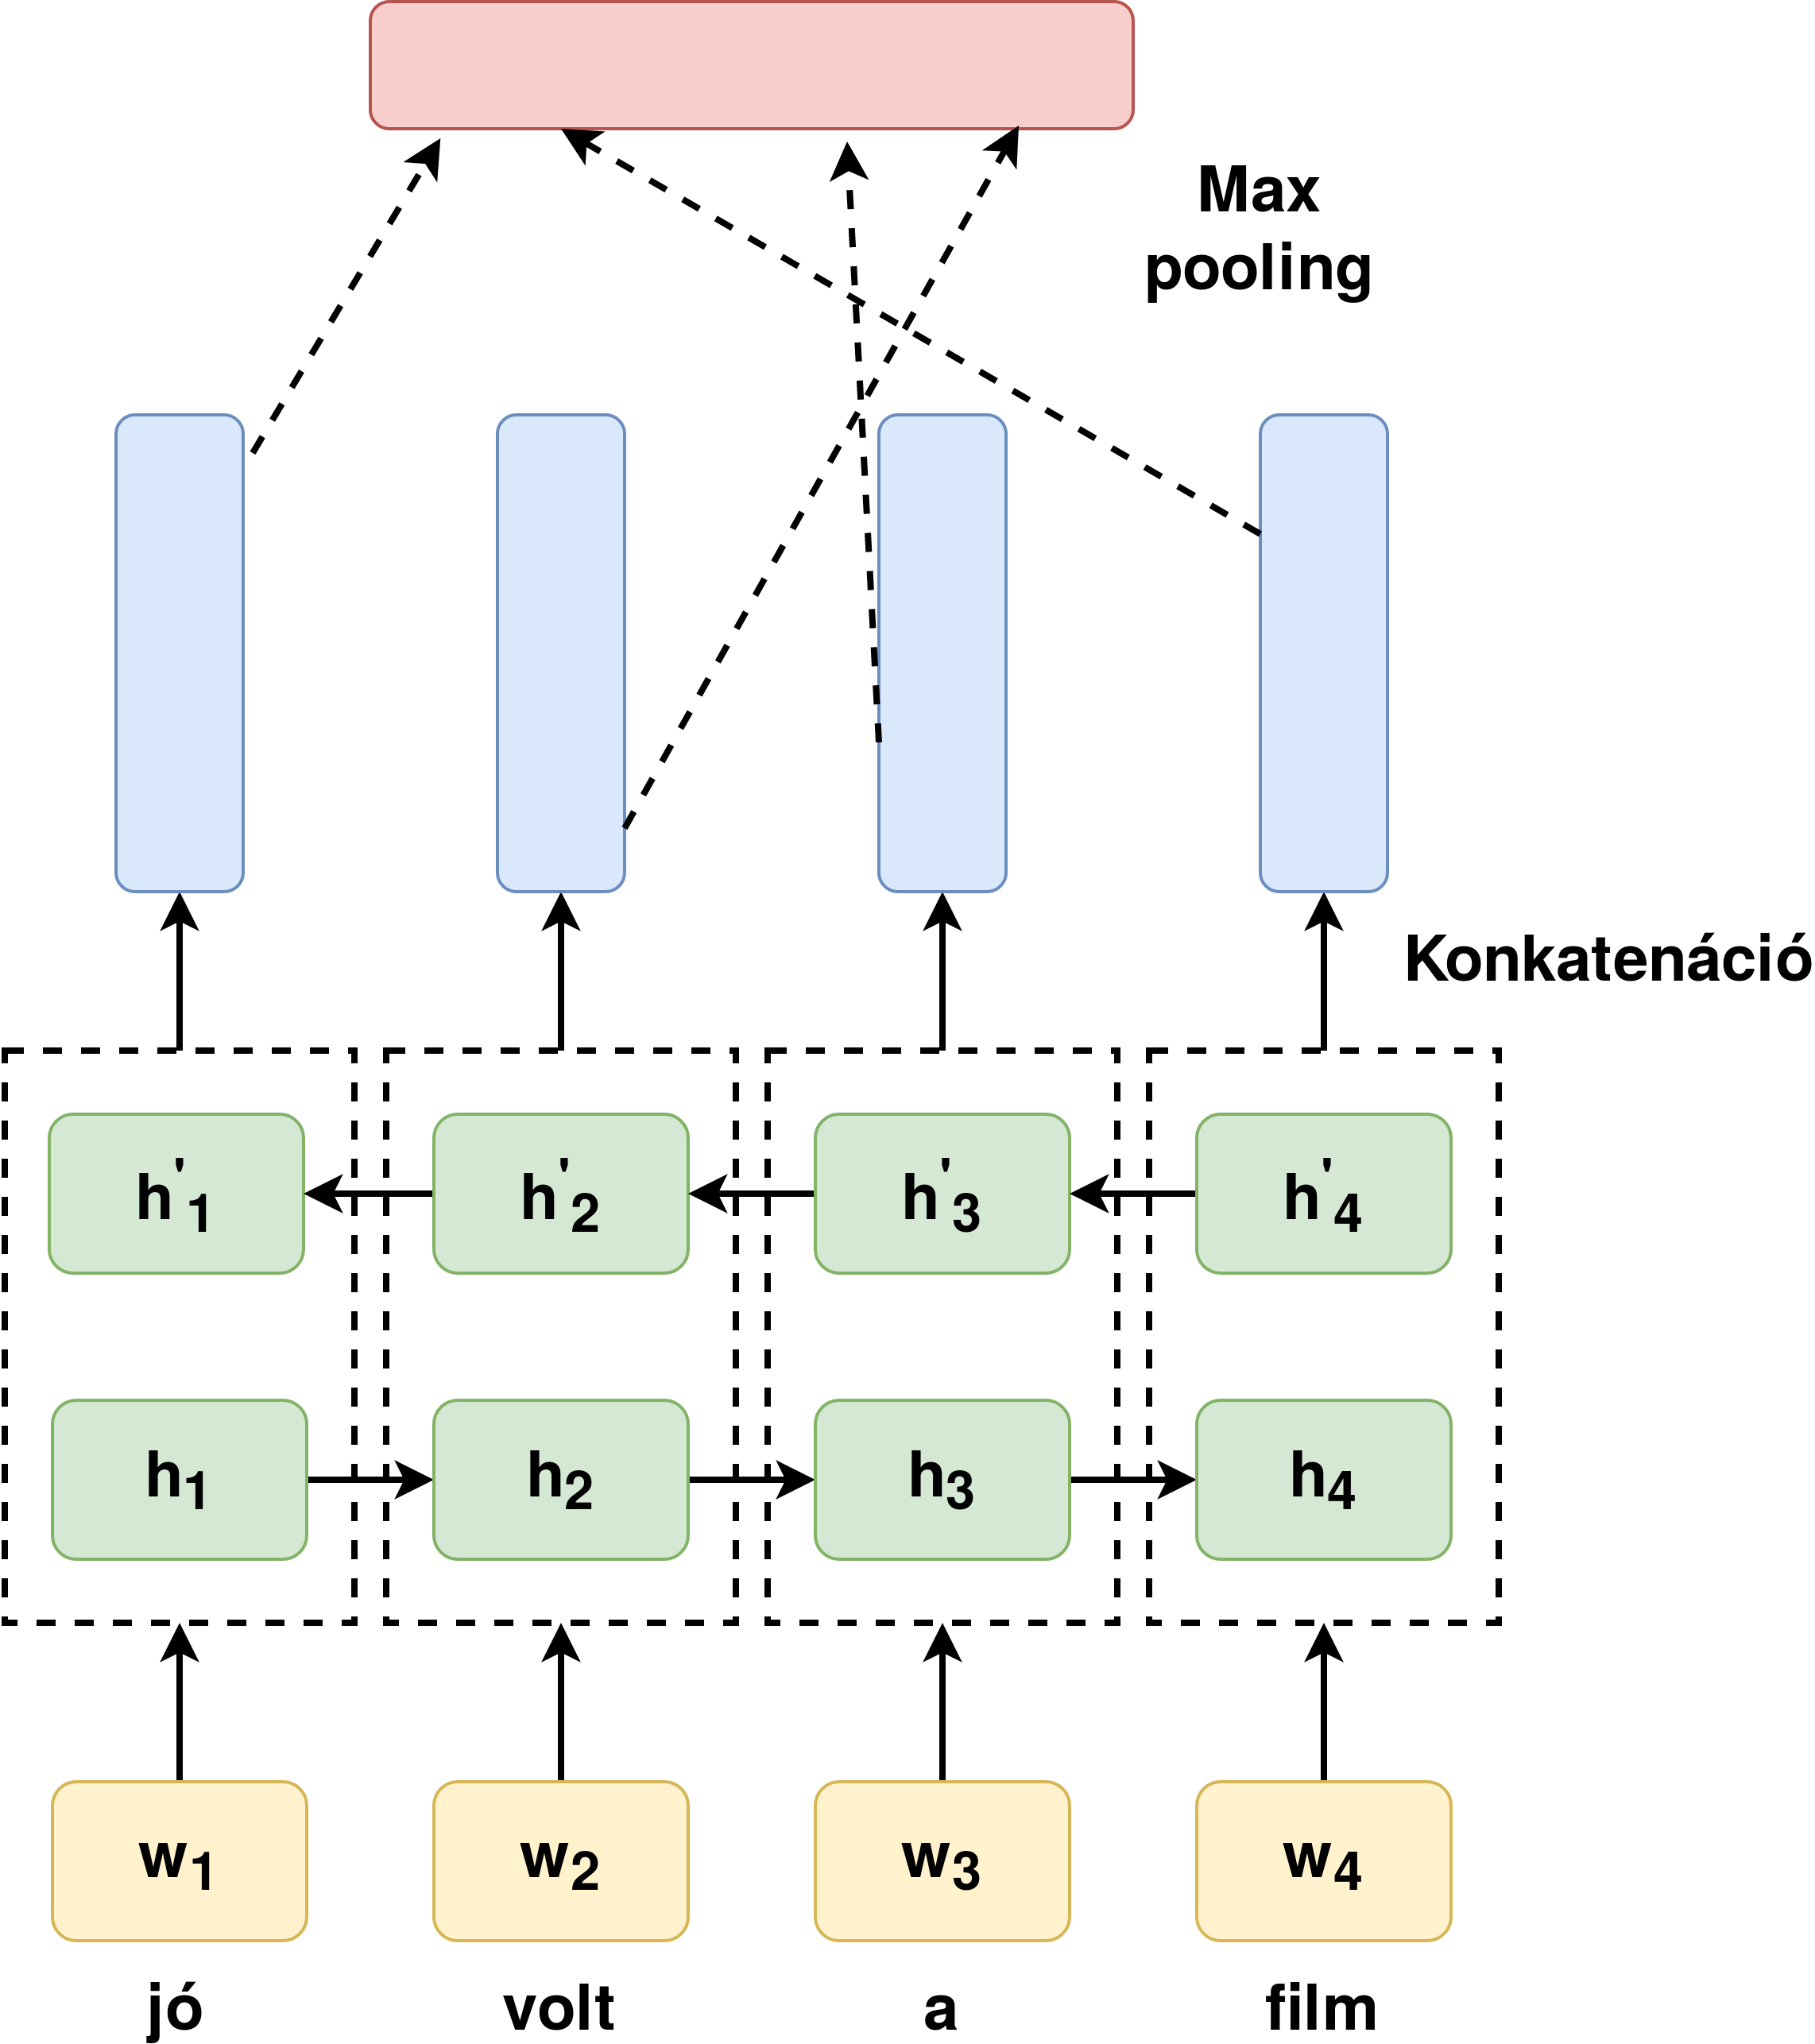
\includegraphics[width=0.45\textwidth,height=180px]{biLSTM-max-pooling}
	\caption{A BiLSTM + max pooling architektúra}
\end{figure}

A sűrű rétegek tanítása közben az egyes neuronok között kialakulhatnak keresztfüggőségek, így túltanulhat a modellünk az adott adathalmazra. A \textit{dropout} egy olyan regularizációs technika, amely kikényszeríti, hogy az egyes neuronok önállóan tanuljanak, így véd a túltanulás ellen és a neurális háló is jobban fog generalizálni. A tanítási fázis során az összes iteráció, összes batch-e esetén minden neuron és hozzá tartozó aktiváció $1-p$ valószínűséggel véletlenszerűen kidobásra kerül. A teszt fázis alatt az összes neuron cselekvőképes, de az aktivációkat a helyes működés miatt $p$ állandóval szorozni kell. Bár a tanítási idő minden epoch során kevesebb lesz, a dropout körülbelül duplázza a konvergációhoz szükséges iterációk számát. A reprezentáció tanulására szolgáló neurális háló mindkét LSTM rétegére konfigurálható \textit{dropout}-ot alkalmaztam.

\begin{figure}[H]
	\centering
	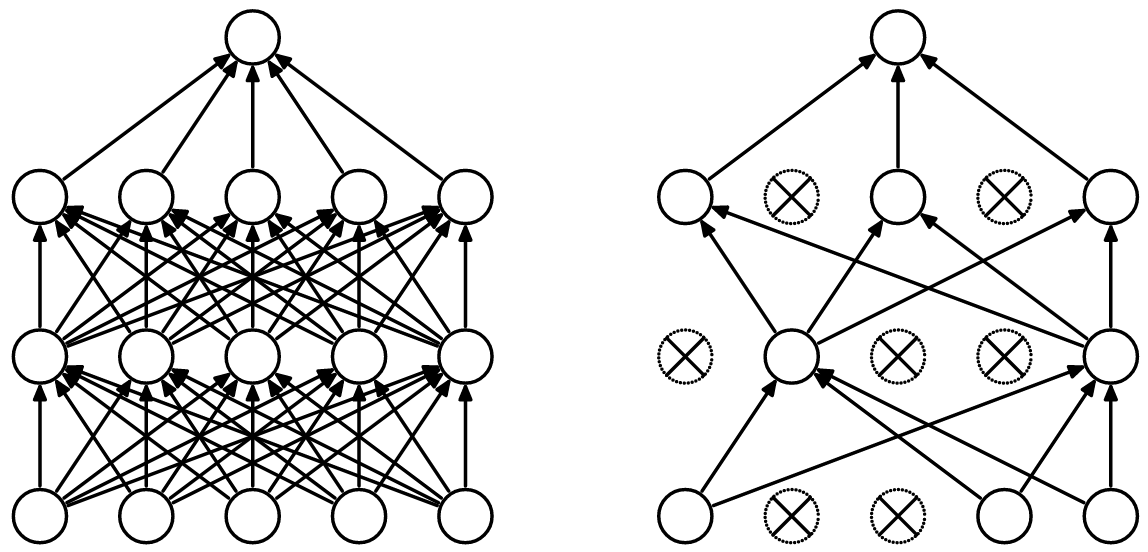
\includegraphics[width=0.6\textwidth,height=140px]{dropout}
	\caption{A dropout vizualizációja}
\end{figure}

A BiLSTM réteg által generált szekvenciális kimenet egy \textit{pooling} rétegbe vezet.

\subsection{Pooling réteg}

A \textit{pooling} ötletét szintén a számítógépes képfeldolgozás ágazatától kölcsönözte az NLP. Míg konvolúciós rétegek esetén a \textit{feature map}-ek kisebb szegmensein elvégzendő a \textit{pooling} művelet, addig az NLP-ben vektorokra értendő.
A \textit{max pooling} réteg a kapott bemenet megadott tengelyei mentén választja ki a legnagyobb értékeket. Analóg módon a \textit{mean pooling} az átlagot veszi alapul.

A BiLSTM-ben található rejtett rétegek kimeneteinek páronkénti konkatenációján végzett pooling művelet képes kiválasztani a hasznos információt az egyes token-eket/rész szekvenciákat reprezentáló vektorokból. Az így kapott sorvektor lesz a bemeneti szekvencia végső reprezentációja.

A nyelvi modell neurális hálójának implementációja egy konfigurálható \textit{pooling} réteget tartalmaz, így a megoldás \textit{max} és \textit{mean pooling}-gal, továbbá pooling nélkül is képes dolgozni.

\subsection{Paraméterek és konfigurálhatóság}

A reprezentáció neurális hálójának implementációja során törekedtem a minél széleskörűbb konfigurálhatóságra, így elősegítve a könnyebb testreszabhatóságot és az újrafelhasználhatóságot. 

A felhasználó által állítható, modellre vonatkozó paraméterek a következők:
\begin{itemize}
	\item \textit{use\_embedding\_layer} : Alkalmazzon a háló bemeneti réteget, vagy vektorizált az input.
	\item \textit{word\_embedding\_dim} : A bemeneti szóbeágyazási vektorok mérete.
	\item \textit{num\_hidden} : A végső reprezentáció mérete, a rejtett LSTM rétegek méretének kétszerese.
	\item \textit{dropout\_keep\_prob} : Dropout valószínűség.
	\item \textit{pooling} : \textit{Pooling} fajtája. (Max, Mean)	
\end{itemize}

A neurális háló paraméterezhetősége lehetőséget biztosít arra, hogy az architektúra más típusú bemenettel, más célra is felhasználható legyen. Ezen konfigurációkon felül több, a tanítási folyamathoz kapcsolódó érték is állítható.

\section{Tanítás}

Bár a szemantikus reprezentációs modellek pontosságához jelentősen hozzájárul az alkalmazott architektúra teljesítménye, az elmúlt néhány év során mégis inkább a tanítóhalmazok és a tanítási módszerek felé irányult a figyelem.

A neurális hálóknak a korábbi hagyományos, feladatspecifikus tanítás alatt egyszerre kellett megérteni a dokumentumhalmaz nyelvét és megtanulni az adott feladathoz szükséges ismereteket. A \textit{transfer learning} technika segítségével ez a két folyamat különválasztható. Az előtanulás során feldolgozott nagy mennyiségű adat hatására a háló megragadja az adott dokumentumok nyelvi sajátosságait, így a finomhangolás alatt a modell koncentrálhat csak az adott feladatra. Az eredmény legtöbbször egy jobban működő reprezentáció.

Az előtanítási feladatok olyan jellegű kihívások elé állítják a reprezentáció neurális hálóját, amelyek során egy erős, általános tudást képes megszerezni. A probléma megoldásához implementált feladat a BERT előtanításához hasonló \textit{multi-task learning}. 

A \textit{multi-task learning} több feladaton egyszerre történő tanulást jelent, ami jobb generalizációra készteti a hálót. Az egyik feladat a \textbf{maszkolás}, amely az egyes szavak közötti szemantikai és szintaktikai jelentés ábrázolását támogatja. A másik feladat a \textbf{következő mondat}, mely a mondatok közötti kohézió reprezentációját segíti.

Mivel az említett feladatok számára tanítóadatot bármely célnyelvű korpuszból könnyedén lehet generálni, ezért elméletileg az előtanítás a végtelenségig skálázható. Az input előállítása során a \textit{hungarianWebcorpus} nevű adathalmazzal dolgoztam, mivel az jelentős mennyiségű szöveges adatból áll, és a sorok az OSCAR adathalmazzal ellentétben sorrendtartóak.

A generálás során az algoritmus rögzített tokenszámú szekvenciákra osztotta a korpuszt. Olyan esetben, mikor nem volt elég token a szekvencia kitöltésére – például rövid dokumentumok, dokumentumvégek – , "[PAD]" speciális helykitöltő \textit{padding} token-eket konkatenált a dokumentum szavaihoz. 
 
A maszkolás a BERT-ben alkalmazott technika alapján történt: az előállított token szekvenciák elemeinek 15\%-át véletlenszerűen kiválasztotta. 
\begin{itemize}
	\item A kiválasztott token-ek 80\%-át a "[MASK]" speciális token-nel helyettesítette. 
	\item 10\%-át a szótárból választott véletlenszerű szóval helyettesítette.
	\item A maradék 10\% esetében maradt az eredeti token.
\end{itemize}

A BERT szerzői szerint, ha a maszkolt token-ek 100\%-át prediktálná a rendszer, nem feltétlen lenne képes megfelelő minőségű reprezentációt generálni a nem maszkolt szavaknak. Ha a kiválasztott token-ek 90\%-át maszkolná és 10\%-ot random választott szóval helyettesítene, az arra késztetné a modellt, hogy úgy gondolja, az adott szó soha nem helyes. Ha pedig a kiválasztott token-ek 90\%-át maszkolná és 10\% maradna az eredeti szó, a modell lemásolná a nem kontextusfüggő beágyazásokat.

A \textit{következő mondat} feladathoz szükséges "mondatpárokat" az így előállított tokenszekvenciákon végigiterálva generálta az algoritmus. $S$ szekvenciát $0.5$ valószínűséggel $S$ után következő szekvenciával, $0.5$ valószínűséggel a korpuszból választott véletlenszerű szekvenciával konkatenálta. A két szekvencia közé egy speciális "[SEP]" mondathatárt jelző token-t illesztett. A végső adathalmaz az így kapott A[SEP]B alakú maszkolt, fix méretű szekvenciákból álló halmaz, mely mérete $13.3$ GB.

\begin{note}
A "mondat" szó ebben az esetben token-ek tetszőleges méretű sorozatát jelenti.
\end{note}
 
A bemenet előállításához szükség volt arra az információra, hogy maximum hány token hosszúságú szekvenciákra darabolja az algoritmus a dokumentumokat és mi a minimális soronkénti token-szám, amelyet még elfogadjon. 

\begin{figure}[H]
	\centering
	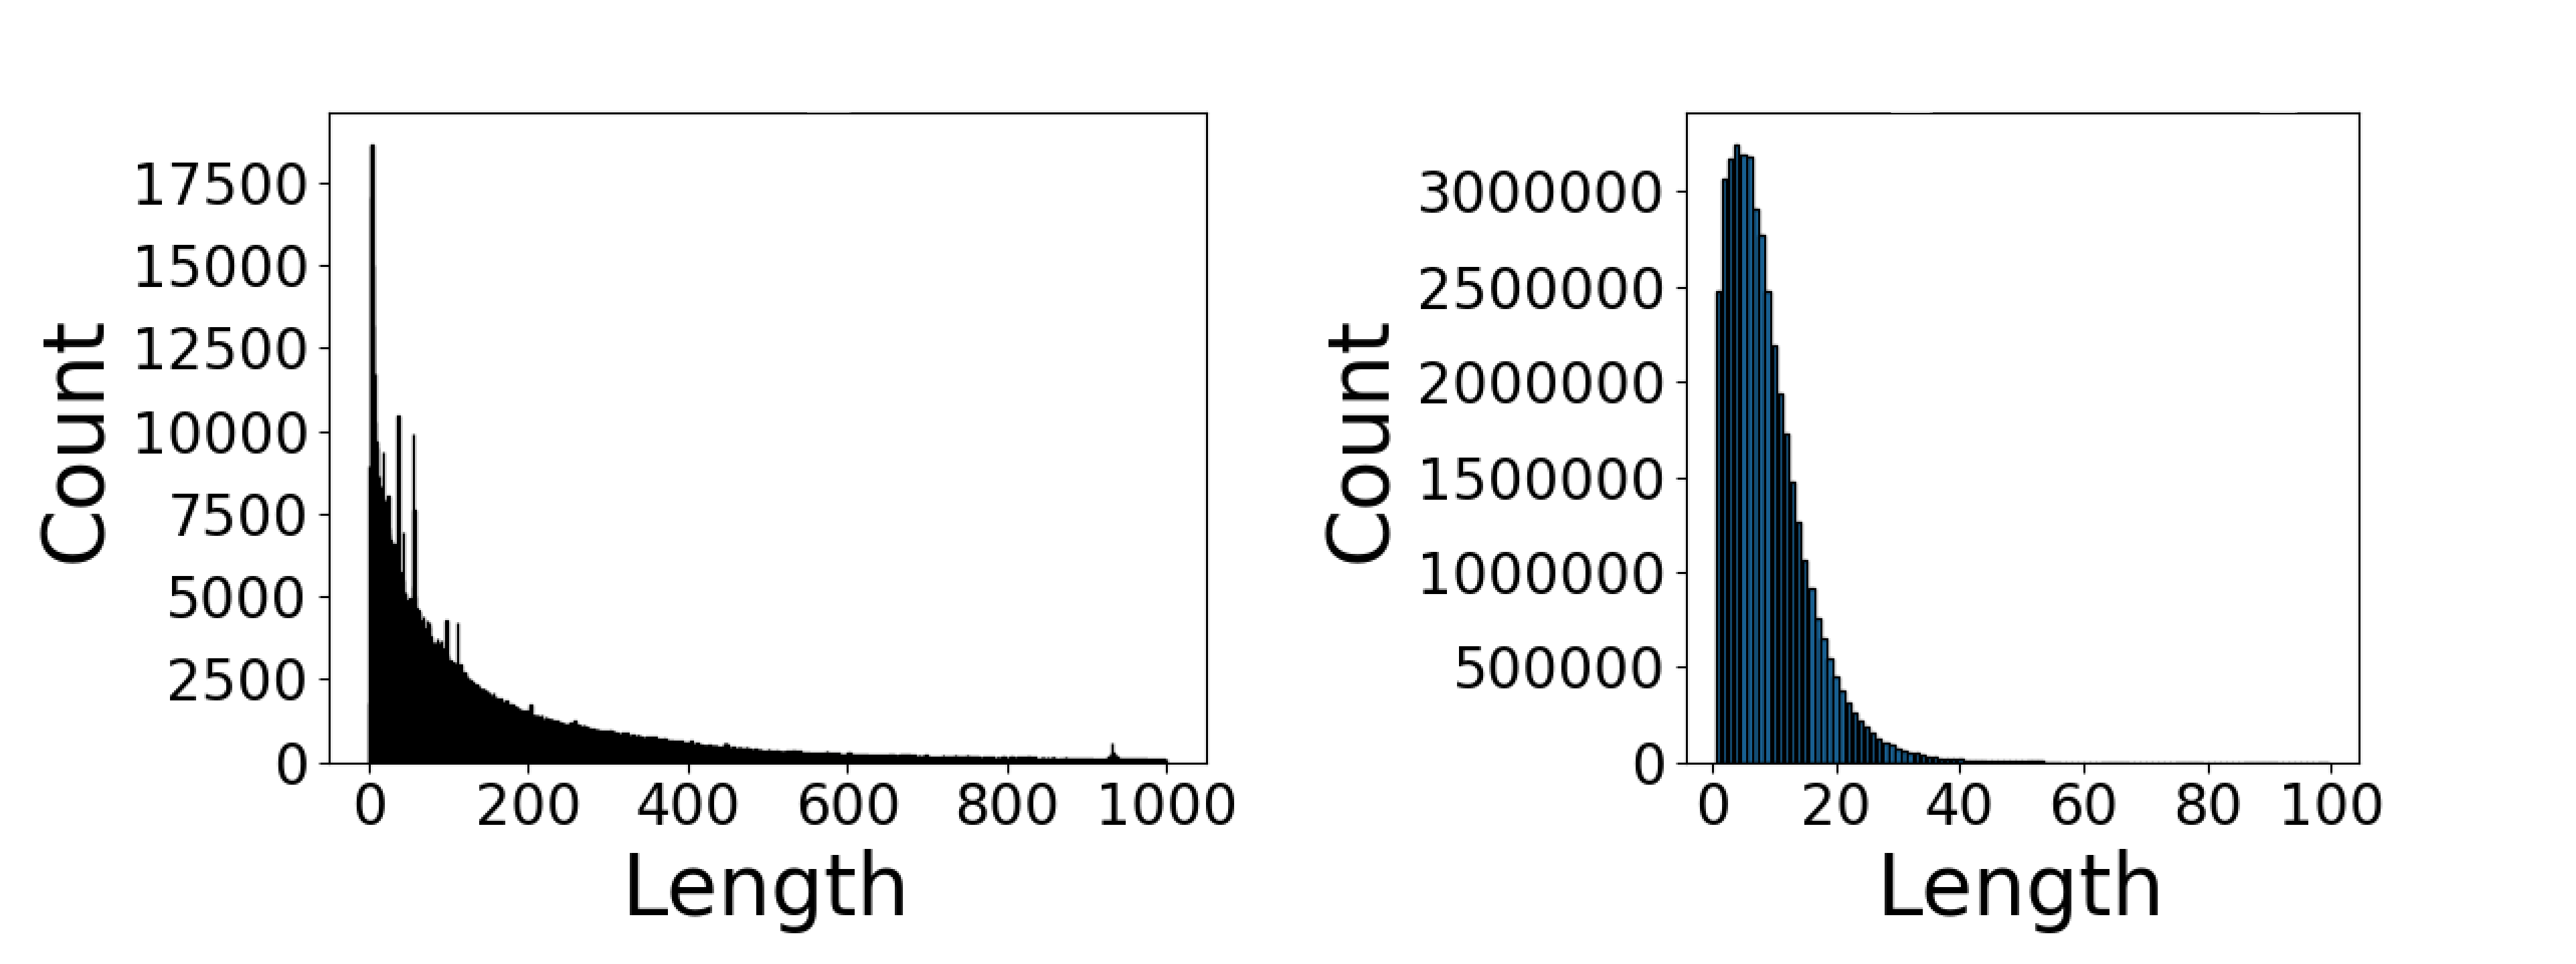
\includegraphics[width=1\textwidth,height=180px]{docLengths}
	\caption{Az 1000 token alatti dokumentumok száma (balra); A 100 token alatti dokumentumok száma (jobbra)}
\end{figure}

\begin{figure}[H]
	\centering
	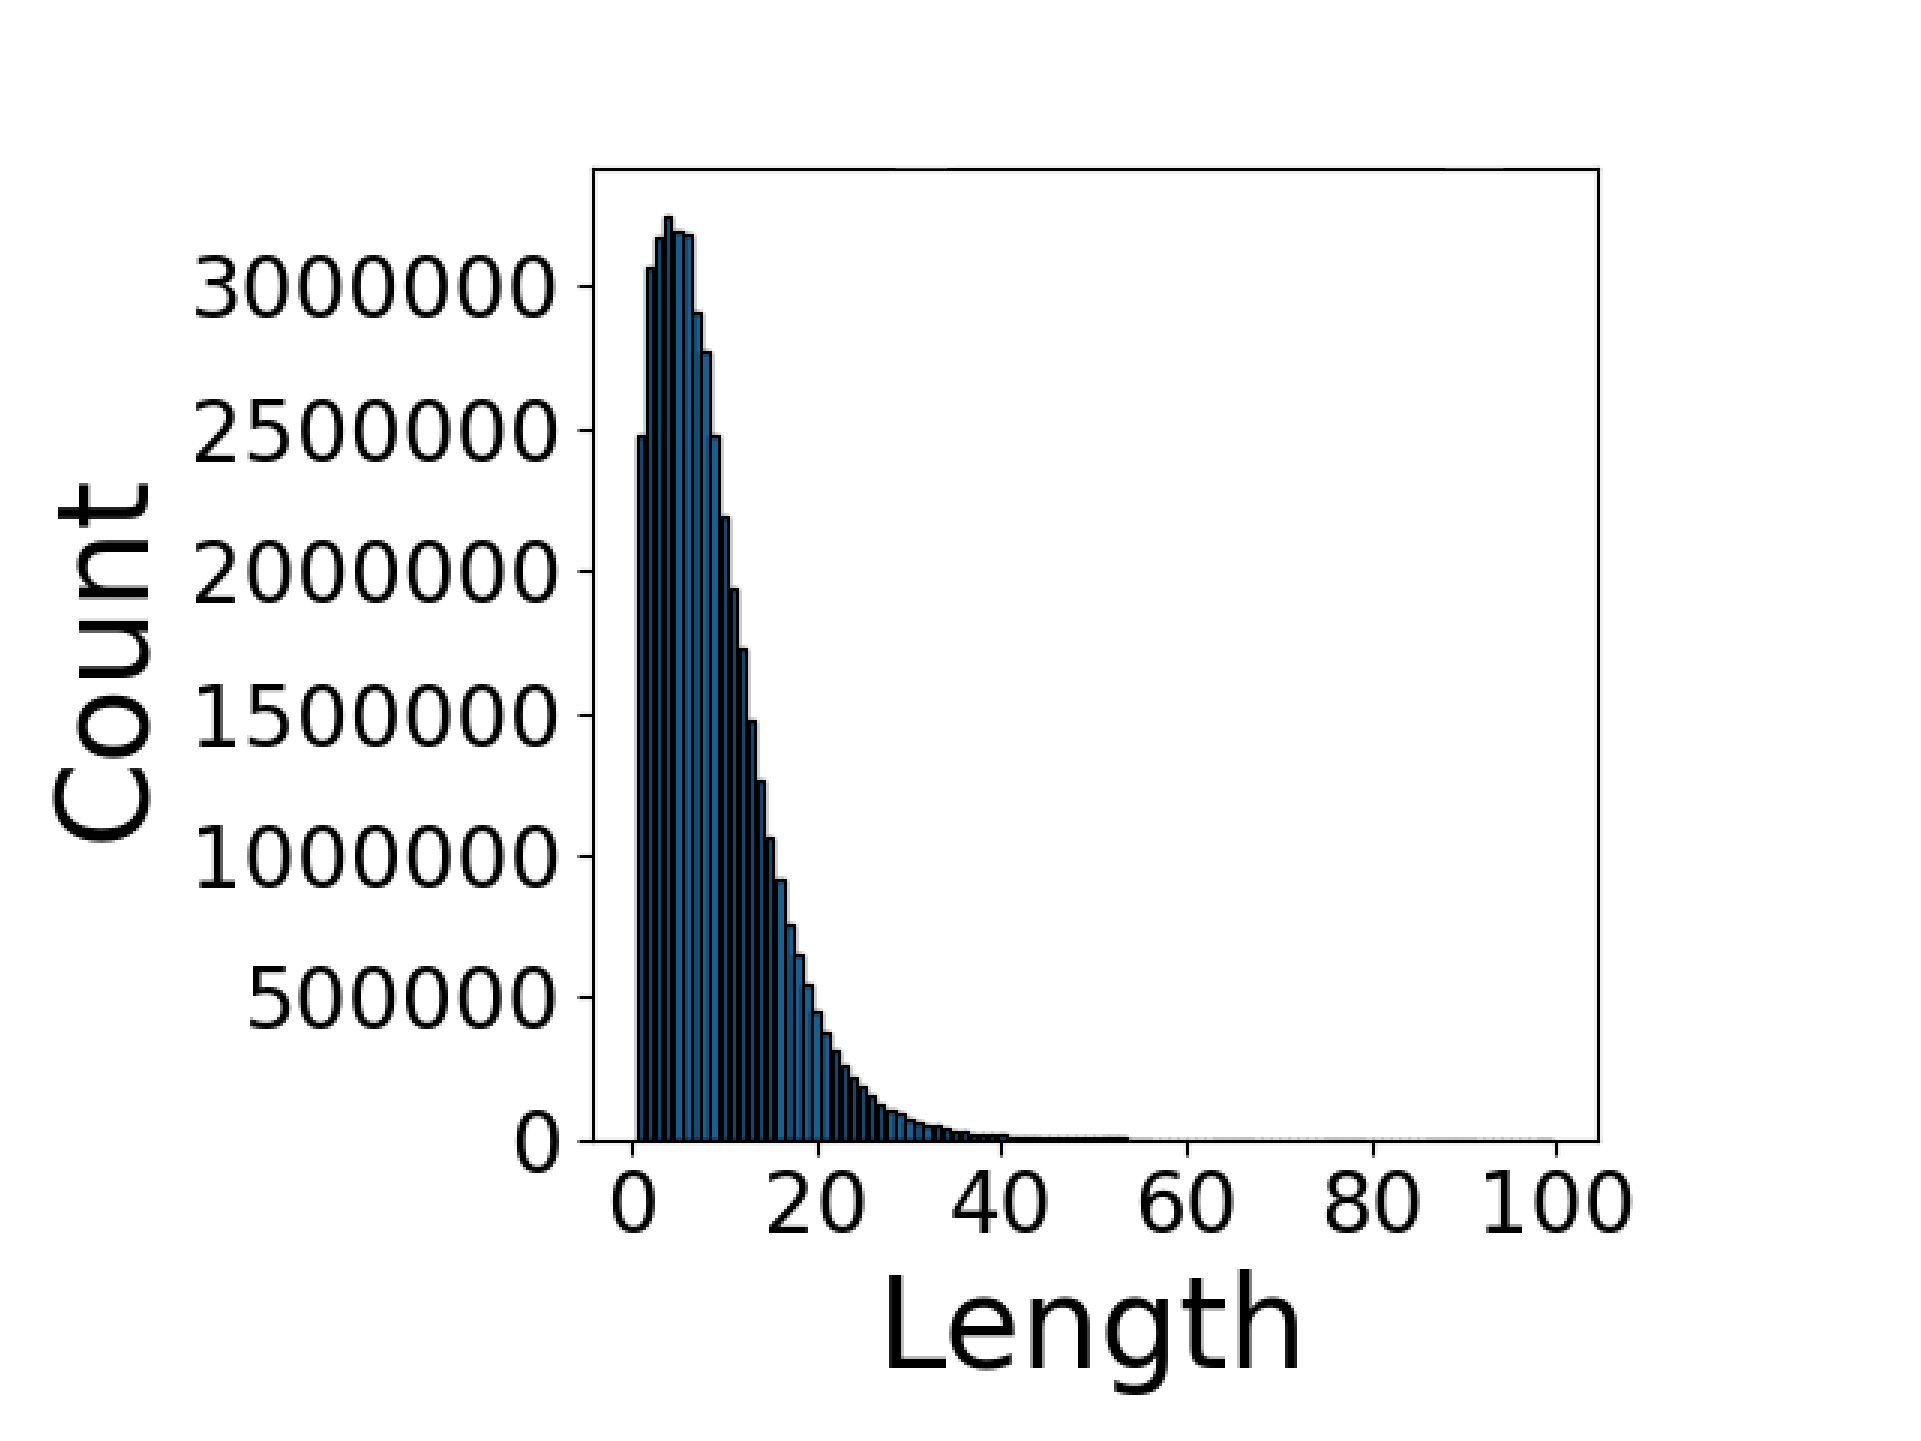
\includegraphics[width=0.6\textwidth,height=180px]{lineLengths}
	\caption{Az 50 token hosszúság alatti mondatok}
\end{figure}

A dokumentumokra és a dokumentumok soraira vonatkozó mérések alapján minimális token-számnak 10-et, maximális szekvenciahossznak 100-at határoztam meg. A cél az volt, hogy a lehető legtöbb információt sikerüljön kinyerni a dokumentumokból és csak relatíve kevés esetben kelljen \textit{padding}-ot alkalmazni, továbbá ne legyen a konfigurációnak teljesíthetetlen memóriaigénye. A végső bemeneti hossz így 201 lett.

Bemeneti réteg használata esetén a neurális háló inputjára a mondatpárok token-jeinek Word2Vec azonosítója kerül. Az \textit{embedding lookup} művelet ezen azonosítók segítségével választja ki a réteg számára átadott beágyazási mátrixból az adott token-ekhez tartozó szóvektorokat. Felmerülhet a kérdés, hogy mi történik a speciális token-ekkel ebben az esetben. A speciális token-eket a Word2Vec modell nem ismeri, így azok nem kerültek be a beágyazási mátrixba sem. A probléma megoldására bevezettem a meglévő Word2Vec dimenziók mellé minden egyes speciális token számára egy saját dimenziót és a hozzá tartozó azonosítókat. Ezen tokeneket reprezentáló vektorok kiterjedése a saját dimenziójukban 1, az összes többi dimenzióban 0. Így a speciális vektorok merőlegesek a többi vektorra és azonosan 1 távolságra kerültek tőlük. Ennek okán a speciális token-ek nem befolyásolják a tanulás során a szemantikai információkat. A bemeneti rétegnek átadott beágyazási mátrix mérete – az [UNK], Word2Vec modell által nem ismert szavakat jelölő token-nel együtt – $(\text{word\_embedding\_dim} + 4) \times \text{szótár méret} $ lesz.

Bár a \textit{maszkolás} és a \textit{következő mondat} feladatok megosztják egymással a bemeneti réteget és a modellt a \textit{multitask learning} során, a feladatok megoldásához használt fejek és a feladatspecifikus bemenetek különböznek.

\subsection{Maszkolás feladat}

A maszkolási feladat során a neurális háló célja kitalálni, milyen token-ek voltak a [MASK] token-ek helyén. A feladat abszolválásához a fejnek szüksége van a mondatpárok generálása során létrejött egyéb információra is. Ilyen információ a maszkolt token-ek szekvencián belüli pozíciója, Word2Vec azonosítója és súlya. Mivel a [MASK] token-ek megfelelő eloszlása érdekében az algoritmus a [PAD] token-eket is letakarja, ezért fontos a súlyok bevezetése. Egy maszkolt token súlya 0 lesz, ha a token eredetileg [PAD] token volt, egyébként 1. 

A fej a BiLSTM háló \textit{pooling} nélküli, szekvenciális kimenetével dolgozik. A kimenetből kiválasztja a maszkolt szavak reprezentációit. Az így kapott \textit{num\_hidden} hosszú vektorokat egy sűrűn kapcsolt, GELU aktivációval \cite{gelu} ellátott rétegen vezeti át, melynek kimeneti mérete megegyezik a kibővített Word2Vec modell beágyazási dimenziójával. Majd a sűrű rétegtől kapott kimenetet megszorozza a beágyazási mátrixszal, annak érdekében, hogy az egyes vektorok a szótár dimenziójába kerüljenek, továbbá \textit{log softmax} aktivációt alkalmaz, hozzájutva a maszkolt token-ekre vonatkozó valószínűségek logaritmusához a teljes szótárra nézve. A feladat tanítási \textit{loss} függvénye az egyes eredeti token-ekre vonatkozó logaritmusok összegének ellentettjének átlaga.


\subsection{Következő mondat feladat}

A \textit{következő mondat} feladat alatt a neurális hálónak ki kell találnia, hogy A[SEP]B bemenet esetén B szekvencia A rákövetkezője-e. A tanítás során a fej számára biztosítani kell a szekvenciákhoz tartozó címkéket. Ezen címkéket a bemeneti adathalmazt előállító algoritmus generálja. Előfordulhat olyan eset, mikor az algoritmus nem tud az adott dokumentumból A mondat mellé B mondatot választani, mert a dokumentum túl rövid, vagy éppen dokumentumhatárra ért. Ekkor értelemszerűen minden esetben hamis lesz a címkéje az adott bemeneti szekvenciának. Ez a működés kiegyensúlyozatlansági problémához vezethet, melyet az algoritmusban alkalmazott számláló hatékonyan ki tud védeni. Ha többségbe kerül a negatív esetek száma, az algoritmus 1 valószínűséggel pozitív eseteket generál. 

\begin{note}
	A jobb megértés érdekében a dolgozathoz mellékeltem egy példa bemenetet.
\end{note}

A fej a BiLSTM háló \textit{max pooling} utáni vektoriális kimenetével, tehát a mondatokat reprezentáló vektorokkal dolgozik. A mondatvektorokra klasszikus bináris klasszifikációt alkalmaz, azaz egy sűrűn kapcsolt rétegen vezeti át őket, melynek kimenete 2 széles és az aktivációs függvénye a \textit{log softmax}. A feladat tanítási \textit{loss} függvénye az így kapott logaritmusok összegének ellentettjének átlaga lesz.

\subsection*{Tanítás - folytatás}
A \textit{multitask learning} során a neurális háló egyszerre két feladatot próbál megoldani, így jobban generalizál. A háló az SGD (\textit{Stochastic Gradient Descent}) nevű algoritmus segítségével minimalizálja a globális \textit{loss} függvényt, amely a két feladat \textit{loss} függvényének összege.
Az SGD számára implementáltam egy konfigurálható \textit{decay} algoritmust. A \textit{learning rate decay} a \textit{loss} függvény értékének \textit{epoch}-onkénti túl lassú csökkenése esetén öttel osztja a \textit{learning rate}-et, így elérve a jobb konvergációs képességet. Az algoritmus minden \textit{epoch} során menti a \textit{transfer} számára szükséges súlyokat és a tanítás aktuális állapotát is.

A jól paraméterezhető tanítás érdekében az implementáció során törekedtem a minél széleskörűbb konfigurálhatóságra. A következő tanításra vonatkozó értékeket állíthatja a felhasználó:
\begin{itemize}
	\item \textit{batch\_size} : A tanításhoz használt \textit{minibatch}-ek mérete.
	\item \textit{num\_inputs} : Az input vektorok mérete.
	\item \textit{num\_time\_steps} : A bemenet szélessége.
	\item \textit{min\_sentence\_length} : A legkisebb token-szám amit az algoritmusnak figyelembe kell vennie.
	\item \textit{max\_sentence\_length} : Az egyes mondatok \textit{padding} utáni hossza.
	\item \textit{masked\_lm\_prob} : A token-ek maszkolási valószínűsége.
	\item \textit{max\_predictions\_per\_seq} : A legnagyobb maszkolható tokenszám egy mondatpár esetén.
	
	\item \textit{learning\_rate\_start} : A \textit{learning rate} kezdőértéke.
	\item \textit{lr\_decay} : \textit{Learning rate decay} ki/be.
	\item \textit{lr\_decay\_threshold} : Az előző és az aktuális \textit{epoch loss} érték mekkora különbsége estén ossza le a \textit{learning rate}-et öttel. Az alapérték 0, tehát ha magasabb, vagy ugyan akkora az aktuális \textit{epoch loss} érték, mint az előző.
	\item \textit{epochs} : Az adathalmazon történő iterációk száma.
	\item \textit{mask\_padding} : Maszkolja-e a \textit{padding} karaktereket.
\end{itemize}

tanítási részletek 2 modell


\section{Vektorok generálása}



mentett súlyok betöltése, súlyok fagyasztása, fej nélküli használat

%két kép kicserélése